%!TEX root = paper.tex
% Template for PLoS
% Version 1.0 January 2009
%
% To compile to pdf, run:
% latex plos.template
% bibtex plos.template
% latex plos.template
% latex plos.template
% dvipdf plos.template

\documentclass[10pt]{article}
%\documentclass[aps,twocolumn]{revtex4-1}
%\documentclass[aps,twocolumn]{article}
% \usepackage{multicol}

% amsmath package, useful for mathematical formulas
\usepackage{amsmath}
\setcounter{MaxMatrixCols}{50}
% amssymb package, useful for mathematical symbols
\usepackage{amssymb}

% graphicx package, useful for including eps and pdf graphics
% include graphics with the command \includegraphics
\usepackage{graphicx}

% cite package, to clean up citations in the main text. Do not remove.
\usepackage{cite}

\usepackage{color}

% Use doublespacing - comment out for single spacing
%\usepackage{setspace}
%\doublespacing

% Text layout
\topmargin 0.0cm
\oddsidemargin 0.5cm
\evensidemargin 0.5cm
\textwidth 16cm
\textheight 21cm

% Bold the 'Figure #' in the caption and separate it with a period
% Captions will be left justified
\usepackage[labelfont=bf,labelsep=period,justification=raggedright]{caption}

% Remove brackets from numbering in List of References
\makeatletter
\renewcommand{\@biblabel}[1]{\quad#1.}
\makeatother

% Leave date blank
\date{}

\pagestyle{myheadings}
%% ** EDIT HERE **

\usepackage{bussproofs}

% xy-pic for diagrams
\usepackage[all]{xy}
% subcaption
\usepackage{subcaption}
% hyperref
%\usepackage[linkbordercolor={.67 .27 .27},citebordercolor={.09 .29 .54},urlbordercolor={.09 .29 .54}]{hyperref}
\usepackage{hyperref}
\hypersetup{colorlinks=true,
linkcolor=[rgb]{.67 .27 .27},
citecolor=[rgb]{.09 .29 .54},
urlcolor=[rgb]{.09 .29 .54}}

% color table cells http://goo.gl/ZmpJv
\usepackage[table]{xcolor}
% rotate text in table http://goo.gl/Lb4Zd
\usepackage{rotating}
% listings for code highlighting in appendix
\usepackage{listings}
\usepackage{setspace}
%!TEX root = ../plos_template.tex
% http://widerin.org/blog/syntax-highlighting-for-python-scripts-in-latex-documents
\definecolor{Code}{rgb}{0,0,0}
\definecolor{Decorators}{rgb}{0.5,0.5,0.5}
\definecolor{Numbers}{rgb}{0.5,0,0}
\definecolor{MatchingBrackets}{rgb}{0.25,0.5,0.5}
\definecolor{Keywords}{rgb}{.67, .27, .27}
\definecolor{self}{rgb}{0,0,0}
\definecolor{Strings}{rgb}{.09,.29,.54}
\definecolor{Comments}{rgb}{0,0.5,0}
\definecolor{Backquotes}{rgb}{0,0,0}
\definecolor{Classname}{rgb}{0,0,0}
\definecolor{FunctionName}{rgb}{0,0,0}
\definecolor{Operators}{rgb}{0,0,0}
\definecolor{Background}{rgb}{0.98,0.98,0.98}

\lstnewenvironment{python}[1][]{
\lstset{
numbers=left,
numberstyle=\footnotesize,
numbersep=1em,
xleftmargin=1em,
framextopmargin=2em,
framexbottommargin=2em,
showspaces=false,
showtabs=false,
showstringspaces=false,
frame=l,
tabsize=4,
% Basic
basicstyle=\ttfamily\small\setstretch{1},
%basicstyle=\ttfamily\footnotesize,frame=single,#1,
backgroundcolor=\color{Background},
language=Python,
% Comments
commentstyle=\color{Comments}\slshape,
% Strings
stringstyle=\color{Strings},
morecomment=[s][\color{Strings}]{"""}{"""},
morecomment=[s][\color{Strings}]{'''}{'''},
% keywords
morekeywords={import,from,class,def,for,while,if,is,in,elif,else,not,and,or,print,break,continue,return,True,False,None,access,as,,del,except,exec,finally,global,import,lambda,pass,print,raise,try,assert},
keywordstyle={\color{Keywords}\bfseries},
% additional keywords
morekeywords={[2]@invariant},
keywordstyle={[2]\color{Decorators}\slshape},
emph={self},
emphstyle={\color{self}\slshape},
%
}}{}

\usepackage{placeins}
\usepackage{longtable}
\usepackage{dot2texi}
\usepackage{tikz}
\usetikzlibrary{automata,shapes,arrows}
% todo notes see http://www.texample.net/tikz/examples/todo-notes/
\usepackage[colorinlistoftodos]{todonotes}
\usepackage{amsthm}
\usepackage{bibunits}

% hyperref with bibunits
% http://tex.stackexchange.com/a/101495/6784
% \makeatletter
% \def\hyper@natlinkstart#1{%
%   \Hy@backout{#1}%
%   \hyper@linkstart{cite}{cite.\@bibunitname.#1}%
% %                             ^^^^^^^^^^^^^^
%   \def\hyper@nat@current{#1}%
% }

% \def\hyper@natlinkbreak#1#2{%
%   \hyper@linkend#1\hyper@linkstart{cite}{cite.\@bibunitname.#2}%
% %                                             ^^^^^^^^^^^^^^
% }

% \def\hyper@natanchorstart#1{%
%   \hyper@anchorstart{cite.\@bibunitname.#1}%
% %                         ^^^^^^^^^^^^^^
% }

% \def\bibcite#1#2{%
%   \@newl@bel{b}{#1}{\hyper@@link[cite]{}{cite.\@bibunitname.#1}{#2}}%
% %                                             ^^^^^^^^^^^^^^
% }%

% \def\@lbibitem[#1]#2{%
%   \@skiphyperreftrue
%   \H@item[\hyper@anchorstart{cite.\@bibunitname.#2}%
% %                                 ^^^^^^^^^^^^^^
%   \@BIBLABEL{#1}\hyper@anchorend\hfill]%
%   \@skiphyperreffalse
%   \if@filesw
%     \begingroup
%       \let\protect\noexpand
%       \immediate\write\@auxout{%
%         \string\bibcite{#2}{#1}%
%       }%
%     \endgroup
%   \fi
%   \ignorespaces
% }%

% \def\@bibitem#1{%
%   \@skiphyperreftrue\H@item\@skiphyperreffalse
%   \hyper@anchorstart{cite.\@bibunitname.#1}\relax\hyper@anchorend
% %                         ^^^^^^^^^^^^^^
%   \if@filesw
%     \begingroup
%       \let\protect\noexpand
%       \immediate\write\@auxout{%
%         \string\bibcite{#1}{\the\value{\@listctr}}%
%       }%
%     \endgroup
%   \fi
%   \ignorespaces
% }%

% \def\@citex[#1]#2{%
%   \let\@citea\@empty
%   \@cite{%
%     \@for\@citeb:=#2\do{%
%       \@citea
%       \def\@citea{,\penalty\@m\ }%
%       \edef\@citeb{\expandafter\@firstofone\@citeb}%
%       \if@filesw
%         \immediate\write\@auxout{\string\citation{\@citeb}}%
%       \fi
%       \@ifundefined{b@\@citeb}{%
%         \mbox{\reset@font\bfseries ?}%
%         \G@refundefinedtrue
%         \@latex@warning{%
%           Citation `\@citeb' on page \thepage \space undefined%
%         }%
%       }{%
%         \hyper@natlinkstart{#2}%
% %       ^^^^^^^^^^^^^^^^^^^^^^^^
%             \hbox{\csname b@\@citeb\endcsname}%
%         \hyper@natlinkend%
% %       ^^^^^^^^^^^^^^^^^^
%       }%
%     }%
%   }{#1}%
% }%

% \makeatother
% end - hyperref with bibunits

% define colors
\definecolor{DeepRed}{rgb}{.82,.14,.16}
\definecolor{DeepBlue}{rgb}{0,0.36,0.62}

% set depth for table of contents
% http://tex.stackexchange.com/a/17879/6784
% http://tex.stackexchange.com/a/11669/6784
\setcounter{tocdepth}{4}
\setcounter{secnumdepth}{0}

%% ** EDIT HERE **
%% PLEASE INCLUDE ALL MACROS BELOW

\newtheorem{theorem}{Theorem}[section]
\newtheorem{lemma}[theorem]{Lemma}

\theoremstyle{definition}
\newtheorem{definition}[theorem]{Definition}
\newtheorem{example}[theorem]{Example}
\newtheorem{xca}[theorem]{Exercise}

\theoremstyle{remark}
\newtheorem{remark}[theorem]{Remark}


% Set autoref text
% http://tex.stackexchange.com/a/36576/6784
\renewcommand*{\figureautorefname}{Fig.}
\renewcommand*{\equationautorefname}{Eq.}
\renewcommand*{\tableautorefname}{Table}

\renewcommand{\refname}{References}

\newcommand{\beginsupplement}{%
        \setcounter{table}{0}
        \renewcommand{\thetable}{S\arabic{table}}%
        \setcounter{figure}{0}
        \renewcommand{\thefigure}{S\arabic{figure}}%
     }

\def\tr{\mathrm{tr}}
\def\Path{\mathrm{Path}}
\def\hier{\mathbf{Hier}}
\def\Vertex{\mathrm{Vertex}}
\def\adj{\mathrm{adj}}
\def\wprod{\mathbf{wp}}
\def\length{\mathbf{len}}
\def\connectivity{d}
\def\reffigexamplesystemmodules{\ref{fig:modsccsym}A}
\def\reffigscc{\ref{fig:modsccsym}B}
\def\reffighiertransformations{\ref{fig:modsccsym}C}
\def\reffigrobustconnect{\ref{fig:combined}A}
\def\reffigrobusthierarchy{\ref{fig:combined}B}
\def\reffigconnectcycle3D3x3{\ref{fig:combined}C}
\def\reffigconnectdist3D3x3{\ref{fig:combined}D}
%% END MACROS SECTION


\begin{document}

% Add Figure, Table prefixes to references
% http://tex.stackexchange.com/a/6063/6784
\let\ref\autoref

% Remove prefix of footnote
% \makeatletter
% \renewcommand{\thempfn}{\thefootnote}
% \makeatother

\pagenumbering{arabic}

\title{\bf Hierarchical Network Structure Promotes Dynamical Robustness}

\author{Cameron Smith$^{1}$,
Raymond S. Puzio$^{1}$,
Aviv Bergman$^{1,2,3,4,*}$}

\affiliation{$^1$Department of Systems and Computational Biology,\\
$^2$Dominick P. Purpura Department of Neuroscience,\\
$^3$Department of Pathology, Albert Einstein College of Medicine,\\
1301 Morris Park Ave, Bronx, NY 10461, USA\\
$^4$Santa Fe Institute, 1399 Hyde Park Road, Santa Fe, NM 87501, USA
\\
$*$to whom correspondence should be addressed: aviv@einstein.yu.edu}

\date{\today}

%!TEX root = ../paper.tex
% The analysis of dynamical systems that attempts to model chemical reaction, gene-regulatory, population, and ecosystem networks all rely on models having interacting components. When the details of these interactions are unknown for systems of interest, one effective approach is to study the dynamical properties of an ensemble of models determined by constraints that can be considered to apply to all such systems. Here we analyze the stability and robustness of a large class of dynamical systems. In particular, we precisely determine the probability distribution of robustness over system connectivity, which has significant implications from the study of metabolic to gene-regulatory to ecosystem network dynamics, for systems with two and three interacting components. We show that robustness is classified by the number of links between strongly connected components of the graph representing the underlying system connectivity leading to the conclusion that the most robust systems are also the most hierarchical. We also demonstrate that permutation of strongly connected components is a fundamental symmetry of dynamical robustness. This results in the classification of the dynamical robustness of biological networks based upon a purely topological property.

\begin{abstract}
The relationship between network topology and system dynamics has significant implications for unifying our understanding of the interplay among metabolic, gene-regulatory, and ecosystem network architecures. Here we analyze the stability and robustness of a large class of dynamics on such networks. We determine the probability distribution of robustness as a function of network topology and show that robustness is classified by the number of links between modules of the network. We also demonstrate that permutation of these modules is a fundamental symmetry of dynamical robustness. Analysis of these findings leads to the conclusion that the most robust systems have the most hierarchical structure. This relationship provides a means by which evolutionary selection for a purely dynamical phenomenon may shape network architectures across scales of the biological hierarchy.
\end{abstract}


\maketitle

% \section{Todo}
% \listoftodos
% \tableofcontents

\begin{bibunit}[pnas]

% \section{Introduction}
%!TEX root = ../paper.tex
The traditional approach taken in the study of chemical reaction, gene-regulatory, population, and ecosystem networks is to derive a system of differential equations to model a particular biological network, attempt to fit that model to data and adjust the modeling assumptions along with parameter values until a good fit is achieved \cite{Meyer2014}. All of these models utilize essentially equivalent mathematical structures \ref{fig:biomodelexamples} \cite{RossCr2003,Alon2006,Palsson2006,HamidBolouri2008,Palsson2011a,Voit2012,Sauro2012}. Developing unified mathematical descriptions of all of these is one of the paramount goals of systems biology.

Recent work has demonstrated that as a result of inhomogeneity in the geometry of the sensitivity of the dynamics over the parameter space for such models, this approach allows for a large variety of models to fit the data \cite{Brown2003,Gutenkunst2007,Daniels2008a,Machta2013,Hines2014,Prabakaran2014,Tonsing2014}. In addition, there is often uncertainty about the very structure of such biological networks. In this context, it is crucial to gain insight into what dynamical phenomena are possible to observe within a given class of dynamical systems, which is necessary to understand in order to determine whether or not a particular dynamical phenomenon should be regarded as unique or generic in the development and investigation of models applied to particular systems \cite{Gunawardena2013,Gunawardena2014}. This can be achieved using a method common in statistical physics involving the consideration of an ensemble of systems that, in comparison to one another, appear to have components that are randomly interlinked.

Indeed, investigating generic properties of a large class of dynamical systems was the approach taken by May in models of ecosystem dynamics \cite{Gardner1970,May1972}. The class of dynamical systems studied by May is, however, not restricted to ecosystem dynamics and encompasses, among others, the dynamics of all of the biological networks represented in \ref{fig:biomodelexamples}. May conjectured on the basis of results from random matrix theory what eventually came to be referred to as the May-Wigner stability theorem \cite{Cohen1984,May1972a,Radius2014}, which implies a relationship between a topological property, system connectivity, and a dynamical property, stability.


% The generic applicability of gaining a better understanding of the class of models investigated by May demonstrates the unequivocal value of deeper investigation.  However, work attempting to continue the development of the so-called May-Wigner stability theorem revealed that May's conjectured stability criterion was not as easy to demonstrate as was initially believed.


% \section{Results}
% %!TEX root = ../paper.tex
Here we determine the relationship between network hierarchy, a topological property, and the probability of \emph{robustness} or \emph{structural stability}, a dynamical property \cite{Smale1967}. Robustness is of interest at all scales of the biological hierarchy, and has been previously studied in the context of gene-regulatory networks \cite{WADDINGTON1942a,VanNimwegen1999,Siegal2002,Ciliberti2007b,Ciliberti2007,Wagner2013}. Intuitively, robustness is the probability of stability to perturbation in the system structure or its parameters for systems which have already been determined to be stable in the sense of linear stability analysis \cite{Davis1962}.

The dynamical model given in terms of a system of differential equations for any network can be represented in terms of an interaction graph (\ref{fig:biomodelexamples} top row). These interaction graphs can be viewed as deriving from the combination of system modules that accept a given pattern of inputs and produce a given pattern of outputs (\reffigexamplesystemmodules). Symmetries are characterized by the ability to interchange these modules or their connectivity without changing some property of the system or its dynamics.

The network architecture can be represented in terms of an adjacency matrix and further abstracted by mapping the interaction graph to the network of strongly connected components (SCCs, see Supplementary Information) (\reffigscc). This map from the interaction graph of a biological network, referred to as $\hier$, has a collection of symmetries shown in \reffighiertransformations. These three symmetries represent transformations that can be performed on the interaction graph that do not change the network of SCCs to which it is associated \reffigscc. Two of these three are also symmetries with respect to dynamical robustness. \ref{fig:robustnesssymmetries} shows an example of these symmetries applied to a specific interaction graph.

We have derived an analytical expression for dynamical robustness as a weighted average of the robustness of the SCCs and the number of links between them that applies to the interaction graph associated to a given dynamical system (Supplementary Material, \ref{eq:sccrobustness}). Examining this expression proves that networks maximizing the number of links between SCCs, will also maximize dynamical robustness (Supplementary Material). This implies that the interaction graphs for systems that are the most robust will also maximize the overall number of SCCs. This analytical result predicts that any biological network whose associated dynamical system has the interaction graph \reffigscc $\,$ top will be more robust than those associated to any of the other interaction graphs in \reffigscc. Because this result is purely topological in nature, it does not depend at all upon any particular details such as the probability distribution from which the component interaction strengths are sampled or the size of the system. The result that dynamical robustness is correlated with system hierarchy therefore applies to an even broader class of dynamical systems than the particular random ensembles we have studied directly.

To test this prediction, we computed the probability distribution of stability and dynamical robustness relative to biological network architecture for ensembles of systems having two or three interacting components (see \ref{tab:structstabmat} and \ref{tab:structstabmat3}). For all of these, we found that robustness is correlated with connectivity, but that the most robust systems have intermediate connectivity for a given network size (\reffigrobustconnect). Accounting for the number of cycles in a network architecture reveals a strong correlation between robustness and connectivity that was hidden when networks with any number of cycles were considered together (\reffigconnectcycle3D3x3). While the most hierarchical network architecture will always lack cycles altogether, cycle number alone is clearly insufficient to account for robustness as the members of each class span nearly the entire range of possible robustness values. Consistent with our analysis of the symmetries of robustness, we found that the most hierarchical network architecture is the most robust (\reffigrobusthierarchy). Moreover, if we consider hierarchy partitioned by connectivity, we find that there is a monotonic increase in robustness following any line of increasing hierarchy in \reffigconnectdist3D3x3.

% \textcolor{red}{We precisely compute the probability of stability and the robustness as a distribution over system connectivity for all systems containing two or three interacting components. We find that stability to structural perturbations of this class of dynamical systems is correlated with connectivity, number of cycles, and the number of links between strongly connected components (SCCs) of the underlying interdependency graph. The latter correlation derives from the fact that the permutation of SCCs is a symmetry of dynamical robustness.}

%!TEX root = ../paper.tex

In the general case of a dynamical system with $n$ components, where the components may be concentrations of chemical species, genes, or biological species, we have an $n$-dimensional vector of state variables or observables $(x_1(t), \ldots x_n(t)) = \vec{x}(t)
$
whose components are solutions to the arbitrary first order system
\begin{equation}\label{eq:eom}
\frac{dx_i(t)}{dt} = F_i(\vec{x}(t), \vec{p}), \; (i=1,\ldots,n)
\end{equation}
where $F=\{F_1,\ldots,F_i,\ldots,F_n\}$ represent, potentially nonlinear, functions of the given vector of state variables and $\vec{p} \in \mathbb{R}^s$ is the vector of $s$ parameters of the $F_i$. These parameters typically represent reaction rates in chemical and gene-regulatory networks, interaction strengths in ecological networks. For example, in the Lotka-Volterra model in \ref{fig:biomodelexamples}, $\vec{x} = (n_1, \ldots, n_N)$, $\vec{p}=(r_1,\ldots,r_N,b_{11},\ldots,b_{NN})$, and $F_i = r_i n_i + \sum_{j=1}^{N} b_{ij} n_i n_j$. The set of all dynamical systems, $\mathcal{D}$, for a given number of state variables $n$ and a given number of parameters $s$, is then
\begin{equation}\label{eq:setdynsys}
\mathcal{D} = \{ (F(-,\vec{p}),\vec{p}) | F \colon \mathbb{R}^n \times \mathbb{R}^s \rightarrow \mathbb{R}^n, \vec{p} \in \mathbb{R}^s \}.
\end{equation}

Fixed points are the simplest class of solutions to the dynamical system characterizing its long-term behavior. If $\vec x$ is a fixed point (i.e. $F_i(\vec{x})=0$ for all $i$), we
may proceed to ask whether it is dynamically stable.
Intuitively, dynamic stability means that, if one chooses the initial
conditions sufficiently close to the fixed point, the solution will
stay nearby.  Physically, this is important because,
if a fixed point ${\vec x}^0$ is unstable, we have zero probability of
observing the solution ${\vec x}(t) = {\vec x}^0$ in the absence of coupling to another system. The Lotka-Volterra model has two fixed points: the trivial one of all zero species $n_i=0$ and the other given implicitly by $r_i + \sum_{j=1}^{N} b_{ij} n_j = 0$. The set of all such fixed points, $\mathcal{F}$, is then
\begin{equation}\label{eq:setfixedpoints}
\mathcal{F} = \{ (d,\vec{x}^0) \; | \; d=(F(-,\vec{p}),\vec{p}) \in \mathcal{D}, \vec{x}^0 \in \mathbb{R}^n,F(\vec{x}^0,\vec{p})=0 \}.
\end{equation}

To determine stability, we linearize the equations of motion (\refsupp{}) about the
fixed point $\vec{x}^0$:
\begin{equation}\label{eq:lineardynsys}
\frac{d\vec{y}(t)}{dt} = A \vec{y}(t),
\end{equation}
where $\vec{y} = \vec{x} - \vec{x}^0$ and the $n \times n$ Jacobian matrix $A$ has components
$$
a_{ij} = \left. \frac{\partial F_i}{\partial x_j} \right|_{\vec{x} = \vec{x}^0}.
$$
The system defined by $F_i$ and $\vec{x}^0$ is dynamically stable if the eigenvalues of $A$ all have real parts less than zero and $A$ is then referred to as a stable matrix (\refsupp{}). This criterion can be checked equivalently in terms of conditions on the coefficients of the characteristic polynomials $\chi(A)$ associated to the systems described by matrices $A$. In the 2-dimensional case, $\chi(A) = z^2 + Tr(A)z+Det(A)$ has solutions $z$ with negative real parts if $Tr(A)<0$ and $Det(A)>0$, which we make use of in examples. Generalized conditions for higher dimensions are available in \cite{Gantmacher1959}. As an example of a Jacobian matrix, the Lotka-Volterra model has
 \begin{equation}\label{eq:lotkavolterrajacobian}
   a_{ij} = \left\{
     \begin{array}{lr}
       r_i + b_{ii} n_i + \sum_{k=1}^{N} b_{ik} n_{k}, & i \neq j\\
       b_{ii} n_i & i=j
     \end{array}.
   \right.
\end{equation}
Evaluation of the stability criterion occurs on a space of two states $\mathcal{S} = \{ S, U \}$ where $S$ stands for stable and $U$ stands for unstable. The stability criterion defines an equivalence relation on the set of all Jacobian matrices $A \in \mathbb{R}^{n \times n}$ deriving from fixed points on $n$ variables that simply splits the set into two classes $S=\{ A \, | \, A \hbox{ is stable}  \}$ and $U~=~\{ A \, | \, A \hbox{ is unstable} \}$.

Jacobian matrices define an equivalence relation, $\sim$, on fixed points given by $(F,\vec{p},\vec{x}^0) \sim (F',\vec{p}\,',\vec{x}^{0'}) $ if and only if
\begin{equation}\label{eq:jaceqrel}
\left. \frac{\partial F(\vec{x},\vec{p})}{\partial \vec{x}} \right|_{\vec{x} = \vec{x}^0} =
\left. \frac{\partial F'(\vec{x},\vec{p}\,')}{\partial \vec{x}} \right|_{\vec{x} = \vec{x}^{0'}}.
\end{equation}
This relation then partitions the set of all fixed points into equivalence classes $\mathcal{F}/{\sim}$, where the class $[A]$ associated to Jacobian matrix $A \in \mathbb{R}^{n \times n}$ is
\begin{equation}\label{eq:jaceqs}
[A] = \left\{ (F,\vec{p},\vec{x}^0) \; | \; \left. \frac{\partial F(\vec{x},\vec{p})}{\partial \vec{x}} \right|_{\vec{x} = \vec{x}^0} = A \right\}.
\end{equation}
An example with two members of $\mathcal{F}$ from each of four different equivalence classes $[A_1]$, $[A_2]$, $[A_3]$, and $[A_4]$ of $\mathcal{F}/{\sim}$ is shown in \ref{fig:robustnessconcept}.

% \subsection{Overview}
The interactions among variables in a dynamical model for any network can be represented in terms of a global interaction graph (\ref{fig:biomodelexamples} top row).
For a general system $X \in \mathcal{D}$ the directed graph $G_X$ that describes the manner in which each of the variables depends upon one another is given by the adjacency matrix $\adj(G_X)$ where $\adj(G_X)_{ij}$ is $1$ if $F_i \hbox{ depends on } x_j$ and $0$ if $F_i \hbox{ does not depend on } x_j$. These two conditions on global system interactions are expressed respectively for all $\vec{x}$ in terms of elements of the Jacobian matrix as $\frac{\partial F_i}{\partial x_j}(\vec{x}) \neq 0$ and $\frac{\partial F_i}{\partial x_j}(\vec{x}) = 0$.
%  \begin{displaymath}
%    \adj(G_X)_{ij} = \left\{
%      \begin{array}{ll}
%        1, & F_i \hbox{ depends on } x_j\\
%        0, & F_i \hbox{ does not depend on } x_j
%      \end{array}.
%    \right.
% \end{displaymath}
For large systems, since any given component is only likely to interact with a relatively small proportion of the other components, these matrices may be sparse.
We can also associate a local interaction graph $G_A$ given by an adjacency matrix $\adj(G_A)$ to each dynamical system having Jacobian matrix $A$ at some fixed point $\vec{x}^0$ where
 \begin{equation}\label{eq:lininterdepadj}
   \adj(G_A)_{ij} = \left\{
     \begin{array}{lr}
       1, & a_{ij} \neq 0\\
       0, & a_{ij} = 0
     \end{array}.
   \right.
\end{equation}
In general, the graph $G_A$ is a subgraph of $G_X$, however, $G_A$ is almost always equivalent to $G_X$ (\refsupp{}). We define the connectivity to be equal to the number of edges in $G_A$, which is equivalent to summing up the number of non-zero entries of $\adj(G_A)$.
These interaction graphs can be viewed as deriving from the combination of system components that accept a given pattern of inputs and produce a given pattern of outputs (\reffigexamplesystemmodules).

Each distinct directed graph $G$, of which there are $k=2^{n(n-1)}$ that could be associated to the interactions in a model defined on $n$ variables, selects a subset of $\mathcal{F} / {\sim}$ (see~\ref{fig:robustnessprocess}C)
\begin{equation}\label{eq:jacgrapheqs}
[G] = \left\{ [A] \; | \; G_A = G \right\}.
\end{equation}
The $G$-classes thereby partition the collection of fixed points, $\mathcal{F}$, over the space of dynamical systems, $\mathcal{D}$, according to the interactions among the variables of the dynamical system represented by the topology of $G$. This partition, $\mathcal{F} / G$, is a coarsening of $\mathcal{F} / {\sim}$.

In the course of biological evolution, the parameter values $\vec{p}$, form of the functions $F$, and environmental conditions restricting access to the basins associated to different fixed points $\vec{x}^0$ corresponding to all different types of networks considered in \ref{fig:biomodelexamples} are subject to, potentially drastic, modifications due to environmental fluctuations. The stochastic process by which these modifications occur induces one on the set of fixed points that results in the assignment of a probability $P(f^T)$ to each history of length $T$, $f^T = ( f_1,f_2,\ldots,f_T ) \in \mathcal{F}^T$.
% $$
% P(f',t+1 | f,t) = \mathcal{T}_{\mathcal{F}}(f',f)
% $$
% for all $f,f' \in \mathcal{F}$.
These dynamics induce a stochastic process on the equivalence classes of fixed points $\mathcal{F}/{\sim}$ indexed by Jacobian matrices given by
$$
P([A]^T) = \sum_{ \{ f^T \mid f_i^T \in [A]_i^T \} } P(f^T)
$$
for each history of length $T$, $[A]^T = ( [A_1], [A_2], \ldots, [A_T] ) \in (\mathcal{F}/{\sim})^T$
% $$
% P([A'],t+1 | [A],t) = \mathcal{T}_{\mathcal{F}/{\sim}}([A'],[A])
% $$
% for all $A,A' \in \mathcal{F}/{\sim}$
as visualized in \ref{fig:robustnessprocess}B. These changes can alter the capacity of a given system to achieve a stable steady state, thereby inducing an even more coarse-grained stochastic process on the stable regions of the space of fixed points given by
$$
P(s^T) = \sum_{ \{ A^T \mid A_i^T \in s_i^T \} } P(A^T)
$$
for each history of length $T$, $s^T = ( s_1, s_2, \ldots, s_T ) \in \mathcal{S}^T$
as visualized in \ref{fig:robustnessprocess}A and B. In order to model this we consider a process whereby perturbations are applied to a given dynamical system and fixed point associated to a stable matrix $A$ leading to $A'$. In order to classify the properties of this process according to network architecture, we enforce the condition $\adj(G_A) = \adj(G_{A'})$, which results in an analogous processes defined on each $G$-class $[G] \in \mathcal{F}/G$ given by
$$
P([A]^T \mid G_A {=} G) = \sum_{ \{ f^T \mid f_i^T \in [A]_i^T \} } P(f^T)
$$
for each history of length $T$, $[A]^T = ( [A_1], [A_2], \ldots, [A_T] ) \in [G]^T$
as visualized in \ref{fig:robustnessprocess}C. This corresponds to an ensemble of dynamical systems with equivalent connectivities, but where each model in the ensemble may otherwise be defined in terms of a different collection of rate functions $F'$, vector of parameters ${\vec{p}}\,'$, or environmental conditions restricting access to $\vec{x}^{0'}$ (\refsupp{}). We then ask, for each distinct network topology on $n$ components, what is the probability, given $A$ is a stable matrix, that $A'$ is also a stable matrix. This quantifies the intuitive statement that, over evolutionary timescales, it is not enough for a system to be stable, but rather that it have a reasonably high probability of remaining stable over continguous timeframes. In terms of a history $s^T$ over the states specifying the stability property, $\mathcal{S}$, this is given by
$$
r = \frac{\sum_{t=0}^{T-1}s_{t+1}^T s_{t}^T}{\sum_{t=0}^{T-1} s_{t}^T},
$$
where we make numerical substitutions for the values of $\mathcal{S}$ such that $S = 1$ and $U = 0$.
Given that the process $P(s^T)$ has stationary probability $P^{\infty}(s)$ for $s \in \mathcal{S}$, the expectation of $r$ as $T \rightarrow \infty$ is approximated by
$$
R = E[r] \approx \frac{\sum_{s,s'} P^{\infty}(s)P^{\infty}(s' \mid s)}{P^{\infty}(S)}.
$$
This conditional probability corresponds to the parameter $R$ of the two-state process depicted in \ref{fig:robustnessprocess}A, and it is what we refer to as dynamical robustness. Comparing the values of $R$ for each $G$-class in $\mathcal{F}/G$ places a partial ordering on network architectures, $G$, which allows for the determination of which network architectures would be expected to be enriched in a process selecting for higher $R$ values.

The network architecture represented in terms of the adjacency matrix, \ref{eq:lininterdepadj}, can be abstracted into modules by mapping the interaction graph to the network of strongly connected components (SCCs, see \refsupp{} and \reffigscc). This map from the interaction graph of a network to its SCCs, referred to as $\hier$ in \ref{fig:modsccsym}, has a collection of intrinsic symmetries shown in \reffighiertransformations{}. These three symmetries, \reffigscc{}, represent transformations that can be performed on the interaction graph that do not change the network of SCCs to which it is associated. Symmetries with respect to some property of the system are characterized by the ability to interchange these modules or their connectivity without changing that property. Two of these three intrinsic symmetries are also symmetries with respect to dynamical robustness. \ref{fig:robustnesssymmetries} shows an example of these latter symmetries applied to a specific interaction graph.

We have derived an analytical expression for dynamical robustness, $R_{tot}$, of a network in terms of its interaction graph as a weighted average of the robustness of the SCCs, $R_i$, the corresponding number of links within each SCC, $d_i$, and the number of links between the SCCs, $l$. The entries of the Jacobian are sampled independently from a generic probability distribution. Examples of vector fields that correspond to this sampling of Jacobian matrices are shown in \ref{fig:robustnessconcept} and \ref{fig:jacobianvectorfields}. The result ultimately holds for the case of simultaneously perturbing any number of elements of the Jacobian. To anchor the intuition before stating the more general result, \ref{eq:robschematic} shows a schematized version for the case of perturbing a single element  (see \reffigscc$\,$ for examples demonstrating this expression)
\begin{equation}\label{eq:robschematic}
R_{tot} = \frac{l+d_1 R_1 + d_2 R_2 + \cdots}{l+d_1 + d_2 + \cdots}.
\end{equation}
For instance, if our graph is the one in \reffigscc{} (middle panels), then we have two connected components, one with two nodes, and one with one node.  From \ref{tab:structstabmat}, we know that the graph with two nodes has probability $0.25$ of being stable and robustness $0.62$.  The graph with one node corresponds to a $1 \times 1$ matrix, so we have probability $0.5$ of stability and robustness $0.5$.  Thus, the probability of our 3-node graph being stable is $0.5 \times 0.25 = 0.125$ and its robustness is computed from \ref{eq:robschematic} in \reffigscc{}, which agrees with the value computed in \ref{tab:structstabmat} up to sampling error.

Examining this expression noting that $R_i$ are all strictly less than one proves that networks maximizing $l$, will also maximize $R_{tot}$.  Given two connected components $C_i$ and $C_j$ with $v_i$ and $v_j$ nodes respectively, we have a maximum of $v_i v_j$ links going from $C_i$ to $C_j$.  Hence, $l \le \sum_{(ij) \in \hier(G)} v_i v_j$.  Since every acyclic digraph can be embedded into a totally ordered
set, we may assume without loss of generality that our components have
been ordered in a way such that, if $(i,j) \in \hier(G)$, then $i <
j$.  Hence, $l \le l_{max}$ where
$$l_{max} = \sum_{i=1}^{n-1}\sum_{j=i+1}^{n}v_i
v_j~=~\frac{1}{2} \left( \sum_{i=1}^{n} v_i \right)^2-\frac{1}{2} \sum_{i=1}^{n}
v_i^2,$$
Hence, we conclude that $R_{tot} \le R_{max}$ where $R_{max}$ is equivalent to \ref{eq:robschematic} with $l_{max}$ substituted for $l$ and the upper bound is attained (\refsupp{}).

This argument also works when we resample more than one entry,
although the notation becomes more complicated.  Suppose that we
resample $m$ nodes.  Define
\begin{widetext}
\begin{equation*}
M = \left\{(m_0, m_1, \ldots, m_n) \,\bigg|\,
m = \sum_{i=0}^n m_i \quad\&\quad
m_0 \le \sum_{i=1}^{n-1} \sum_{j=i+1}^n \ell_{ij} \quad\&\quad
(\forall i \in \{1, \ldots, n\}) \; m_i < \connectivity_i \right\}.
\end{equation*}
\end{widetext}
Then, given $(m_0, m_1, \ldots, m_n) \in M$, there are ${m \choose
m_0, m_1, \ldots. m_n}$ ways of choosing $m_i$ links from $C_i$ and
$m_0$ links between strongly connected components.  Hence, our
weighted average becomes
\begin{widetext}
\begin{equation}
\langle R(\hbox{stab} (G), \mu') \rangle_m =
\frac{\sum\limits_{(m_0, m_1, \ldots m_n) \in M}
      {m \choose m_0, m_1, \ldots. m_n}
      \left(m_0 + \sum\limits_{i=1}^n m_i \langle R(\hbox{stab} (C_i), \mu') \rangle_{m_i} \right)}
     {\sum\limits_{(m_0, m_1, \ldots m_n) \in M}
      {m \choose m_0, m_1, \ldots. m_n} m}
\end{equation}
\end{widetext}

As before, since $\langle R(\hbox{stab} (C_i), \mu') \rangle_{m_i} \le 1$, we may
increase $\langle R(\hbox{stab} (G), \mu') \rangle_m$ by increasing the maximum
possible value of $m_0$ while keeping the strongly connected
components the same.  Again, if we fix $\hier(G)$, the maximum
possible value of $m_0$ is $\sum_{(i,j) \in \hier(G)} v_i v_j$
whereas, if we allow it to vary, the maximum is $\frac{1}{2} ((\sum_{i=1}^n
v_i)^2 - \sum_{i=1}^n v_i^2)$, which is attained when $\hier(G_{max}) =
G_{tot}$.  Hence, we conclude that $\langle R(\hbox{stab} (G), \mu') \rangle_m \le
\langle R(\hbox{stab} (G_{\mathrm{max}}), \mu') \rangle_m$.

This implies that the interaction graphs for systems that are the most robust will maximize the number of links between SCCs as well as the overall number of SCCs with respect to a particular system size. This analytical result predicts that any network whose associated dynamical system has the interaction graph equivalent to the total ordering like that of \reffigscc{} top will be more robust than those associated to any of the other interaction graphs in \reffigscc{}. Because this result is purely topological in nature, it does not depend at all upon any particular details such as the probability distribution from which the component interaction strengths are sampled or the size of the system. The result that dynamical robustness is correlated with network hierarchy therefore applies to an even broader class of dynamical systems than the particular random ensembles we have studied directly.

To test the prediction of this analytical result, we computed the probability distribution of stability and dynamical robustness relative to network architecture for ensembles of systems having two or three interacting components (see \ref{tab:structstabmat} and \ref{tab:structstabmat3}). For all of these, we found that robustness is correlated with connectivity, but that the most robust systems have intermediate connectivity for a given network size (\reffigrobustconnect). Accounting for the number of cycles in a network architecture reveals a strong correlation between robustness and connectivity that was hidden when networks with any number of cycles were considered together (\reffigconnectcycle3D3x3). While the most hierarchical network architecture will always lack cycles altogether, cycle number alone is clearly insufficient to account for robustness as the members of each class span nearly the entire range of possible robustness values. Consistent with our analysis of the symmetries of robustness, we found that the most hierarchical network architecture is the most robust (\reffigrobusthierarchy). Moreover, if we consider hierarchy partitioned by connectivity, we find that there is a monotonic increase in robustness following any line of increasing hierarchy in \reffigconnectdist3D3x3.


% \section{Discussion}
%!TEX root = ../paper.tex
% Our development suggests two predictions that could be used to test the theory described here. One is that,
Our theory predicts that any ensemble of systems where robustness has been positively selected over a sufficiently long period of time should exhibit a bias toward more hierarchical network topologies. For example, at the ecological level, a system subjected to the environmental stress of overfishing, which may imply selection for robustness, has been observed to exhibit such a bias toward more hierarchical network architectures \cite{Bascompte2005}. In the short term, this prediction may be further evaluated at the levels of both metabolic and transcription factor networks, which have already been shown to display hierarchical structure, but whose dynamics have not been sufficiently well characterized to ascertain their robustness \cite{Zhao2006,Bhardwaj2010,Colm}.
%The other prediction of the theory outlined here that may be able to be checked is the converse statement that an ensemble of systems demonstrating a positive or negative bias in their network topology toward hierarchy may have been under selection for, or respectively against, robustness. Of course, in this case, factors other than selection for robustness would not be ruled out by this analysis alone.
In the long term, this prediction may be evaluated using experimental evolution by comparing the degree of hierarchy that emerges in the evolution of gene regulatory network topology in the context of both static and fluctuating environments that differentially select for robustness \cite{Leroi1994}.

%The fact that such a relationship exists has the potential to unify our understanding of biological networks.
In order to further this work from a theoretical perspective, it will be necessary to deepen our understanding of the relationship between dynamical robustness and the underlying network topology.
%One approach is to attempt to compute robustness for systems of larger size. Using existing methods, this would require large-scale Monte Carlo simulations. However,
It may be possible to prove a bound on the robustness of individual SCCs, which could provide more definite knowledge and circumvent the need for expensive simulations. The conservation of robustness with respect to nontrivial symmetries including the interchange of SCCs and permutation within SCCs suggests the existence of an evolutionary neutral space. A deeper mathematical characterization of the full symmetry groupoid of dynamical robustness may thus help to characterize this potential evolutionary constraint \cite{Golubitsky2006}.

The relationship between structure and function is fundamental to networks at every level of the biological hierarchy. Equally fundamental is the ability of systems to persist over long periods of time, which is dependent upon their dynamical robustness. Here we have demonstrated a structure-function relationship wherein biological networks that are more hierarchical are more robust and thus more likely to persist in the evolutionary process.
%Moreover, this result is formulated at a level of abstraction that allows its conclusions to apply independently to each of these levels.


% \section{Methods}
% {\footnotesize
% %!TEX root = ../paper.tex


\section{Reaction Networks, Gene Regulatory Networks, and Ecological Networks with Prescribed Connectivity and Jacobians}\label{sec:reactionnetjacobian}

The quality of interest in this paper is robustness, which is related to the concept of structural stability \cite{Smale1967}, whose evaluation requires the determination of whether or not a given dynamical system that is determined to be stable remains stable under a perturbation to one or more of its defining parameters, its rate functions, or environmental constraints that restrict it to a subset of its basins of attraction. We mean to refer to perturbations to the structure of the system itself as determined by the strengths of the couplings between the components and not only to perturbations of the state vector at a given point in time. It is justified to consider resampling elements of $A$ to generate $A'$ as a proxy for resampling elements of $\vec{p}$ to produce $\vec{p}\,'$ if any matrix $A$ can be obtained for some $F_i$, $\vec{p}$ and $\vec{x}^0$. This holds for the $F_i$ defining the Lotka-Volterra model. This is due to the fact that for a specification of non-zero real numbers for the components of $\vec{x}^0$ and any real numbers for the components of $a_{ij}$, there is a choice of parameters $\vec{p}$ given by $b_{ij} = \frac{a_{ij}}{x_i^0}$ and $r_i = - \sum_{j=1}^n \frac{x_j^0}{x_i^0} a_{ij}$ that generates those particular $a_{ij}$ as the Jacobian matrix of the dynamical system. Checking this property of the domain of realizability of the Jacobian can be done for ensembles of systems other than the Lotka-Volterra ensemble. For arbitrary biochemical reaction and gene regulatory networks, this property is likely to hold so long as not too many types of transformations are constrained from possibility. For example, a simplified version of the general form of the gene regulatory network model presented in \ref{fig:biomodelexamples} center panel is given by the system
\begin{equation}
\frac{dg_i}{dt} = \sum_{j=1}^N k_{ij} g_j,
\end{equation}
with one parameter $k_{ij} \in \mathbb{R}$ for every pair $(g_i,g_j)$ of genes. The Jacobian of this system is $A_{ij} = k_{ij}$, and, therefore, sampling parameters of the model is precisely equivalent to sampling elements of the Jacobian.
% For reaction networks, we demonstrate an ensemble from which arbitrary Jacobians can arise in \ref{sec:reactionnetjacobian}.

To justify our consideration of arbitrary Jacobian matrices in the case of reaction networks, we determine a simple ensemble for which arbitrary Jacobian matrices are realizable. This condition holds if one can solve for the parameter values of the system of equations corresponding to that ensemble in terms of the elements of an arbitrary Jacobian matrix. More precisely, we will show that, given an arbitrary directed graph $G$ where $G_{ii} = 1$ for all $i$, there exists a system of reactions having $G$ as its interaction graph and satisfying the following property: For any point $\vec{x}^0$ in the positive orthant and an arbitrary matrix $M$ whose interaction graph is $G$, there exists a choice of non-negative rates such that $\vec{x}^0$ is a fixed point of the network and the Jacobian equals $M$ at $\vec{x}^0$.

We begin by noting that, since the form of the rate equations for reaction networks are invariant under rescaling the concentrations and rate constants, we can make the coordinates of the point $\vec{x}^0$ be $(1,1,\ldots,1)$.  This will simplify the computation.

Let $N$ be the number of nodes of $G$.  Our reaction net will consist of $N$ species of reactants, $A_1, \ldots, A_N$, whose concentrations are $c_1, \ldots, c_N$.  The reactions are defined as follows:
% \begin{enumerate}
% \item For every integer $1 \le i \le N$, we have the reactions $\emptyset \to A_i$, $A_i \to \emptyset$ and $2A_i \to 3A_i$.
% \item For every pair of integers $1 \le i,j \le N$ such that $G_{ij} = 1$, we have the reactions $A_i + A_j \leftrightarrow A_j$.
% \end{enumerate}
\begin{equation}\label{eq:arbitraryjacobianreactionnetwork}
\begin{aligned}
\emptyset &\to A_i, & 1 \le i \le N,\\
A_i &\to \emptyset, & 1 \le i \le N,\\
2A_i &\to 3A_i, & 1 \le i \le N,\\
A_i + A_j &\leftrightarrow A_j, & i \neq j,\, 1 \le i,j \le N,\, G_{ij} = 1.
\end{aligned}
\end{equation}

The rate equations for such a system are:
% \begin{widetext}
\begin{equation}\label{eq:crnarbitraryjacobian}
\begin{aligned}
\frac{dc_i}{dt} = &F_i = k_{\emptyset \to A_i} - k_{A_i \to \emptyset} c_i + k_{2A_i \to 3A_i} c_i^2 \\
&+ \sum_{\substack{1 \le j \le N \\ j \neq i \\ G_{ij} = 1}} k_{A_j \to A_i + A_j} c_j - k_{A_i + A_j \to A_j} c_i c_j
\end{aligned}
\end{equation}
% \end{widetext}
The Jacobian at $\vec{x}^0$ is given as
% \begin{widetext}
\begin{align*}
\left. \frac{\partial F_i}{\partial c_i}\right|_{\vec{x}^0} &= - k_{A_i \to \emptyset} + 2 k_{2A_i \to 3A_i} - \sum_{\substack{1 \le j \le N \\ j \neq i \\ G_{ij} = 1}} k_{A_i + A_j \rightarrow A_j}, & \\
\left. \frac{\partial F_i}{\partial c_j}\right|_{\vec{x}^0} &= k_{A_j \to A_i + A_j} - k_{A_i + A_j \to A_j}, &
\end{align*}
where $i \neq j$.
% \end{widetext}
By combining the equations $F_i(\vec{x}^0) = 0$ from \ref{eq:crnarbitraryjacobian} and $\frac{\partial F_i}{\partial c_j}|_{\vec{x}^0} = M_{ij}$ we obtain the equivalent system of equations
\begin{align}
& k_{2A_i \to 3A_i} - k_{\emptyset \to A_i} = M_{ii} + \sum_{\substack{1 \le j \le N \\ j \neq i \\ G_{ij} = 1}} k_{A_j \to A_i + A_j} \label{eq:jacobianconstraint1}  \\
& 2k_{2A_i \to 3A_i} - k_{A_i \to \emptyset} = M_{ii} + \sum_{\substack{1 \le j \le N \\ j \neq i \\ G_{ij} = 1}} k_{A_i + A_j \to A_j} \label{eq:jacobianconstraint2}\\
& k_{A_j \to A_i + A_j} - k_{A_i + A_j \to A_j} = M_{ij} \label{eq:jacobianconstraint3}
\end{align}
We may solve these equations for the rate constants as follows.  We begin by solving \ref{eq:jacobianconstraint3} by either choosing $k_{A_i + A_j \to A_j} \ge 0$ and setting $k_{A_j \to A_i + A_j} = M_{ij} + k_{A_i + A_j \to A_j}$ when $M_{ij} \ge 0$ or choosing $k_{A_j \to A_i + A_j} \ge 0$ and setting $k_{A_i + A_j \to A_j} = k_{A_j \to A_i + A_j} - M_{ij}$ when $M_{ij} < 0$.  Pick
% \begin{widetext}
\begin{equation}
\begin{aligned}
k_{2A_i \to 3A_i} \ge \max \bigg(&0, M_{ii} + \sum_{\substack{1 \le j \le N \\ j \neq i \\ G_{ij} = 1}} k_{A_j \to A_i + A_j}, \\
&M_{ii} + \sum_{\substack{1 \le j \le N \\ j \neq i \\ G_{ij} = 1}} k_{A_i + A_j \to A_j} \bigg).
\end{aligned}
\end{equation}
% \end{widetext}
Then we may solve \ref{eq:jacobianconstraint1} for $k_{\emptyset \to A_i}$ and \ref{eq:jacobianconstraint2} for $k_{A_i \to \emptyset}$ and obtain non-negative answers. This demonstrates that arbitrary Jacobian matrices can arise from reaction network ensembles that allow for the possibility of at least those reactions in \ref{eq:arbitraryjacobianreactionnetwork}. Note that \ref{eq:crnarbitraryjacobian}, \ref{eq:jacobianconstraint1}, \ref{eq:jacobianconstraint2}, and \ref{eq:jacobianconstraint3} are linear in the parameter values. Therefore, any probability distribution on the elements of the Jacobian can be obtained from a probability distribution on the parameter values.

\section{Graph associated to the total ordering}\label{sec:totalordering}

A directed graph $G=(V,E)$ is a set $V$ of nodes and a set $E$ of ordered pairs of nodes \cite{Cormen2009}. For example, if $V = \{1,2,3\}$ and $E = \{(1,1),(2,2),(3,3),(1,2),(1,3),(2,3)\}$ then $G=(V,E)$ is the graph depicted in \reffigscc{} top where the labels $1$, $2$, and $3$ have been respectively assigned to the nodes vertically from top to bottom.

 We refer to the most hierarchical network architecture as the directed graph associated to a total ordering on the set of system components corresponding to the set of nodes, $V$, of the graph \cite{Cormen2009}. In general, a totally ordered set is a pair $(S,R)$ consisting of a set $S$ together with a total order relation $R$ on it. An example of a total ordering is the less than or equal to relation, $R \equiv \leq$, on the subset of natural numbers $S \equiv \{1,2,3\}$ given by $R \equiv \{1 \leq 1, 2 \leq 2, 3 \leq 3, 1 \leq 2, 1 \leq 3, 2 \leq 3\}$. The graph associated to this relation is equivalent to the graph shown in \reffigscc{} top and described algebraically in the preceding paragraph. More precisely, the conditions on $R$ for arbitrary elements $x,\,y,\,z \in S$ necessary for $(S,R)$ to be a totally ordered set are
\begin{enumerate}
\item If $x R y$ and $y R x$ then $x=y$ (antisymmetry)
\item If $x R y$ and $y R z$ then $x R z$ (transitivity)
\item $x R y$ or $y R x$ (totality)
\end{enumerate}
The totality condition implies $x R x$ (reflexivity) corresponding to the fact that the directed graph associated to the total ordering has, for each node, an edge whose source and target are the same node.

Corresponding to the SCC decomposition of $G$ we can construct a directed acyclic graph $\hier (G)$ or the condensed graph \cite{Corominas-Murtra2013}.  Each node of $\hier (G)$ corresponds to a strongly connected component of $G$. There is an edge from the node corresponding to component $C$ to the node corresponding to component $C'$ if and only if there exists a link from some vertex in $C$ to some vertex in $C'$ in $G$.  Because of the maximality of strongly connected components, $\hier (G)$ is acyclic.

% One can also perform this construction in the opposite direction.  Start with a directed acyclic graph $A$.  To each node $n$ of $A$ associate
% a strongly connected graph $C_n$.  To each link $(i,j)$ of $A$ associate a non-empty subset of $\Vertex(C_i) \times \Vertex(C_j)$.  The result will be a graph $G$ such that $\hier(G) = A$ and furthermore, every graph $G$ such that $\hier(G) = A$ can be obtained in this manner.

% This map $\hier$ is many-to-one and so there is a large class of
% operations which leaves $\hier(G)$ invariant for a given graph $G$.
% For instance, we may interchange the positions of the strongly
% connected components relative to each other \reffighiertransformations$a$.  Leaving the components fixed, we may move links between nodes in a component \reffighiertransformations$b$ or between components, or even add or delete links \reffighiertransformations$c$.  Some of these operations leave dynamical robustness invariant, so we may regard them as a symmetry groupoid of the systems associated to a given graph $G$ with respect to the robustness property.

% }

\section{Acknowlegements}
%!TEX root = ../paper.tex
Support was provided by NIH MSTP training grant T32-GM007288 to CS, the Fulbright program to XP, and NIH R01-CA164468-01 and R01-DA033788 to AB. The authors would like to thank Jay Sulzberger and Daniel Biro for helpful suggestions and discussion.


% \bibliographystyle{Science}
% \bibliography{bib/books,bib/papers}

\putbib[bib/books,bib/papers]

\pagebreak
\FloatBarrier

\onecolumngrid
\pagebreak
% \section{Figures}
%!TEX root = ../paper.tex

% \begin{figure}[!ht]
% \centering
% \noindent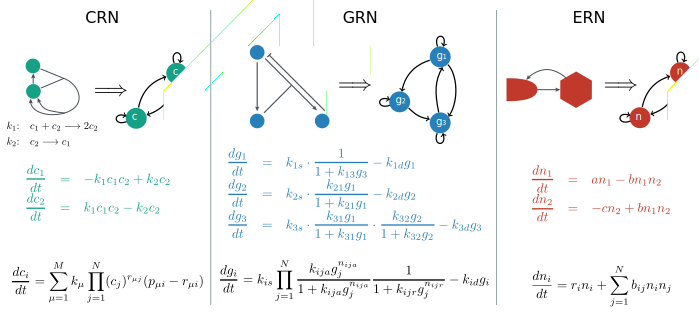
\includegraphics[width=0.9\columnwidth]{fig/biomodelexamples.pdf}
% \caption{{\bf Dynamical models in systems biology.} The top row represents a chemical reaction network (CRN) \cite{Shinar2010}, a gene regulatory network (GRN) \cite{Karlebach2008}, and an ecological regulatory network (ERN) \cite{Rohr2014} in terms of the graphical methods specific to each field mapped into the interaction graph, which provides a unified representation for networks across these fields. The second row represents a particular example of a system of differential equations that are used to model a biological network within each of the domains of application considered here. The third row shows the general form of a system of differential equations that can be used to model any network architecture within each domain.}
% \label{fig:biomodelexamples}
% \end{figure}

% \pagebreak

% \begin{figure}[!ht]
% \centering
% \noindent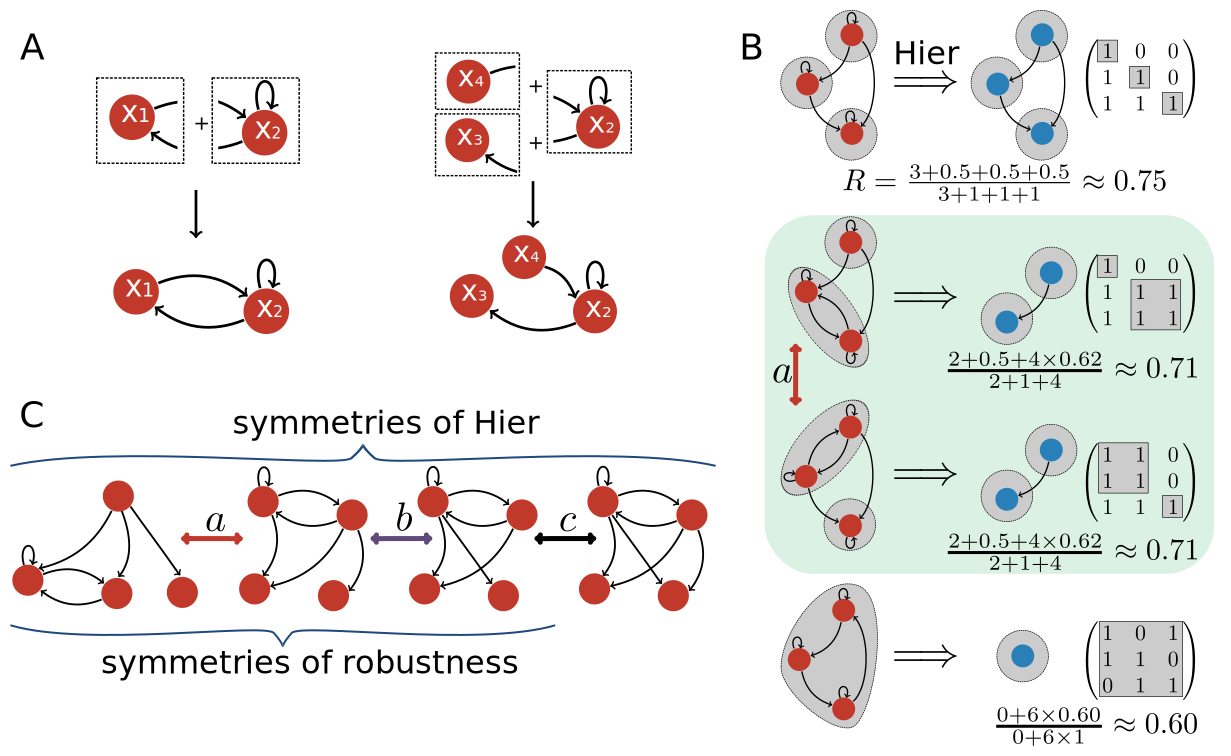
\includegraphics[width=0.9\columnwidth]{fig/modsccsym.pdf}
% \caption{{\bf Open systems, strongly connected components and symmetries of robustness.} (A) Example of the combination of open system modules to construct closed systems. (B) SCCs highlighted in gray for each of the four graphs representing the interdependencies relevant to four different three variable systems. The most hierarchical network, top panel, is the one that maximizes the number of SCCs and the number of links between them. We therefore define hierarchy as $max(\hbox{ED}) - \hbox{ED}$ where ED is the edit distance representing the number of link addition/deletion operations necessary to transform a given graph into the most hierarchical one. The two panels in the middle represent examples of hierarchical modular systems that posess both modularity (i.e. SCCs with more than one variable) and hierarchy. (C) Symmetries of the $\hier$ transformation between graphs and SCCs. The transformation $a$ represents an interchange of SCCs, $b$ moving a link between nodes in a component and $c$ adding a link. All three transformations represent symmetries of the $\hier$ transformation from graphs to SCCs while only $a$ and $b$ are symmetries of robustness.}
% \label{fig:modsccsym}
% \end{figure}

% \pagebreak


% \begin{figure}[!ht]
% \centering
% \noindent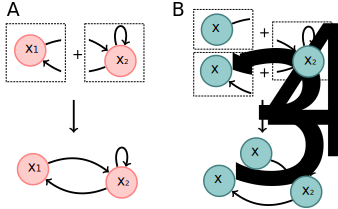
\includegraphics[width=0.4\columnwidth]{fig/examplesystemmodules.pdf}
% \caption{{\bf Example of the combination of open system modules to construct closed systems.} (A) Example of combining two open modules to construct a closed system of two components (B) Analogous example for combining three open modules to construct a closed system with three components}
% \label{fig:examplesystemmodules}
% \end{figure}

% \pagebreak

% \begin{figure}[!ht]
% \centering
% \noindent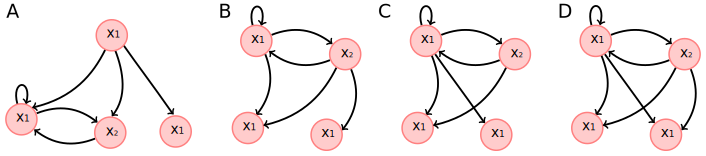
\includegraphics[width=0.7\columnwidth]{fig/hiertransformations.pdf}
% \caption{{\bf Symmetries of the $\hier$ transformation between graphs and SCCs.} The transformation A represents an interchange of SCCs, B moving a link between nodes in a component and C adding a link. All three transformations represent symmetries of the $\hier$ transformation from graphs to SCCs while only A and B are symmetries of robustness.}
% \label{fig:hiertransformations}
% \end{figure}

% \pagebreak

% \begin{figure}[!ht]
% \centering
% \noindent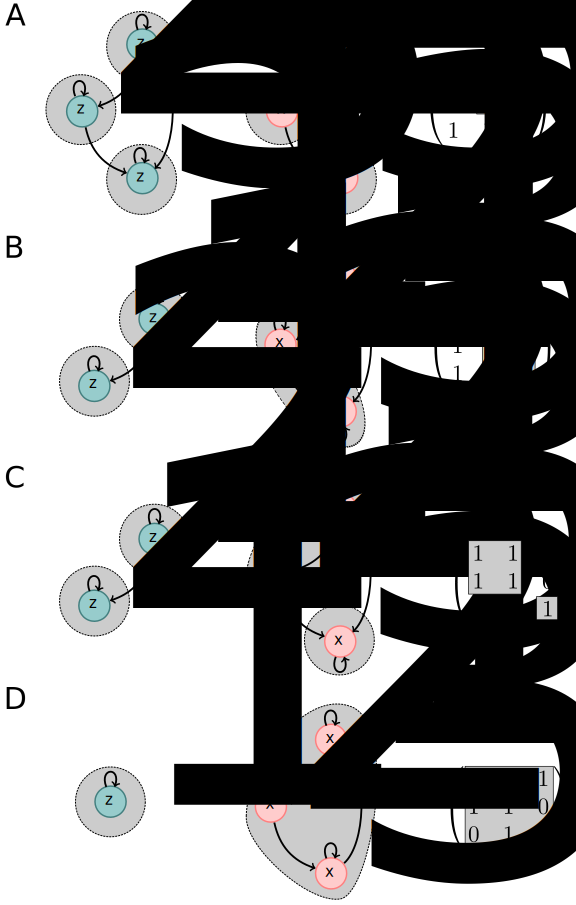
\includegraphics[width=0.4\columnwidth]{fig/scc2.pdf}
% \caption{{\bf Example of strongly connected components.} (A) - (D) show strongly connected components highlighted in gray for each of the four graphs representing the interdependencies relevant to four different three variable systems. Note that the most hierarchical system in (A) has the highest possible number of connected components, three, whereas the system containing a single cycle and therefore posessing no hierarchy contains only one connected component. Systems (B) and (C) represent examples of hierarchical modular systems that posess both modularity and hierarchy.}
% \label{fig:scc}
% \end{figure}

% \pagebreak

% \begin{figure}[!ht]
% \centering
% \noindent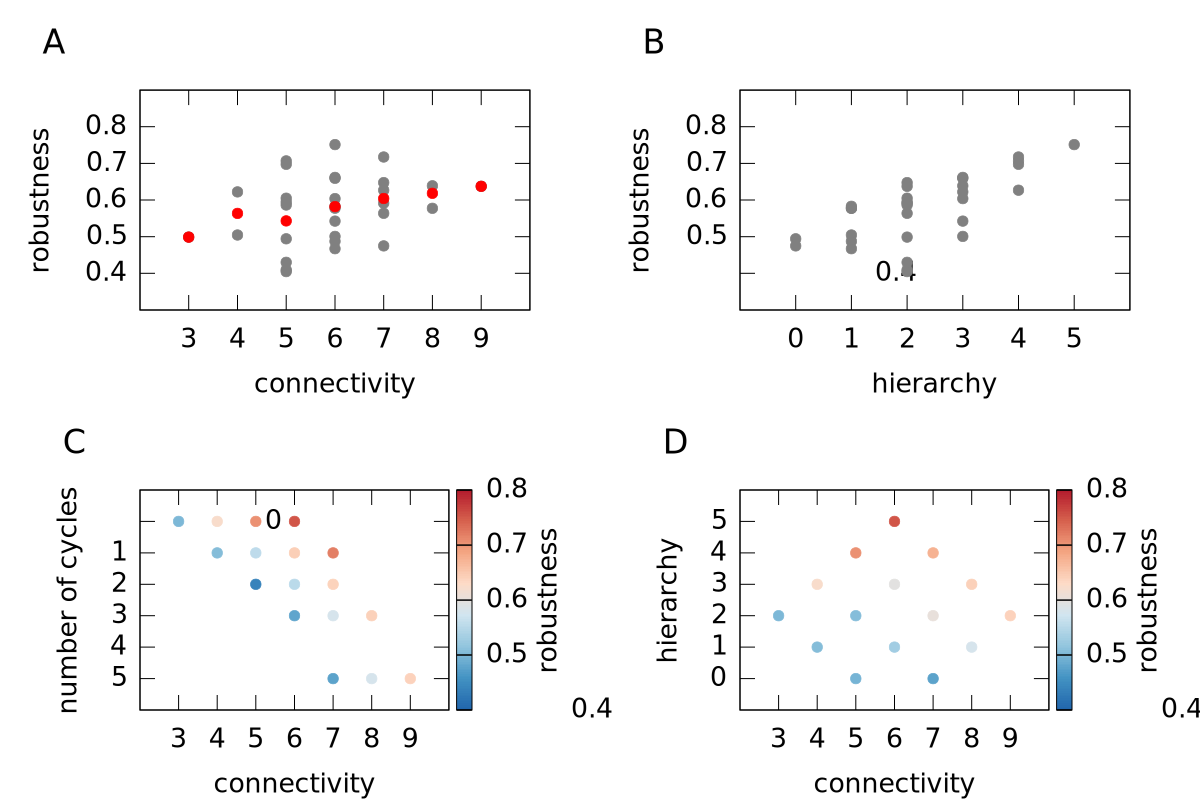
\includegraphics[width=1.0\columnwidth]{fig/combinedfigs.pdf}
% \caption{{\bf Characterization of stability and robustness according to properties of system structure for three variable systems} (A) Robustness versus connectivity. The red line represents a best fit in the least-squares sense with Pearson product-moment correlation coefficient $r=0.29$. The lowest and highest robustness network architectures are labelled. Other network architectures are shown in \ref{tab:structstabmat3}. (B) Robustness versus hierarchy. Correlation coefficient $r=0.67$. (C) Number of cycles and (D) hierarchy vs connectivity and robustness. The color of each point represents the average robustness of all graphs having the parameters specified on the $x$ and $y$ axes.
% }
% \label{fig:combined}
% \end{figure}

% \pagebreak

% \begin{figure}[!ht]
% \centering
% \noindent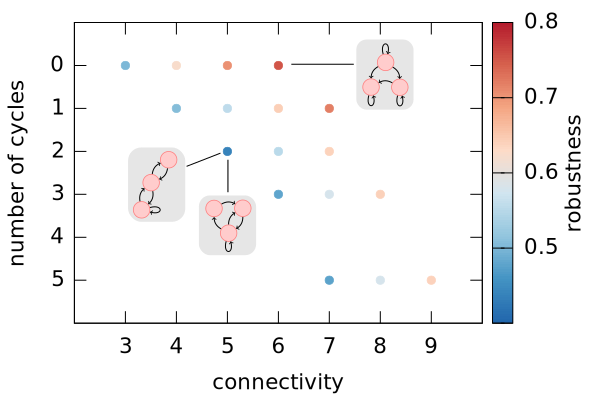
\includegraphics[width=0.8\columnwidth]{fig/connectcycle3D3x3.pdf}
% \caption{{\bf Robustness versus number of cycles and connectivity for three variable systems.} Each point represents the average robustness of all graphs having a given number of cycles and connectivity.}
% \label{fig:connectcycle3D3x3}
% \end{figure}

% \pagebreak

% \begin{figure}[!ht]
% \centering
% \noindent\includegraphics[width=0.8\columnwidth]{fig/connectdist3D3x3.pdf}
% \caption{{\bf Robustness versus hierarchy and connectivity for three variable systems.} Each point represents the average robustness of all graphs having a given hierarchy and connectivity.}
% \label{fig:connectdist3D3x3}
% \end{figure}



\end{bibunit}
\pagebreak
\twocolumngrid

\pagebreak
\FloatBarrier

\beginsupplement
\setcounter{secnumdepth}{4}

\begin{bibunit}[unsrtnat]

\begin{widetext}
\begin{center}
\text{\large \refsupp{} for }\\
\textbf{\large Hierarchical Network Structure Promotes Dynamical Robustness}\\
\text{Cameron Smith, Raymond S. Puzio, Aviv Bergman$^*$}\\
\text{$^*$Corresponding author. E-mail: aviv@einstein.yu.edu}
\end{center}
\end{widetext}

% \section{\refsupp{}}

%!TEX root = ../paper.tex
Here we determine the relationship between network hierarchy, a topological property, and the probability of \emph{robustness} or \emph{structural stability}, a dynamical property \cite{Smale1967}. Robustness is of interest at all scales of the biological hierarchy, and has been previously studied in the context of gene-regulatory networks \cite{WADDINGTON1942a,VanNimwegen1999,Siegal2002,Ciliberti2007b,Ciliberti2007,Wagner2013}. Intuitively, robustness is the probability of stability to perturbation in the system structure or its parameters for systems which have already been determined to be stable in the sense of linear stability analysis \cite{Davis1962}.

The dynamical model given in terms of a system of differential equations for any network can be represented in terms of an interaction graph (\ref{fig:biomodelexamples} top row). These interaction graphs can be viewed as deriving from the combination of system modules that accept a given pattern of inputs and produce a given pattern of outputs (\reffigexamplesystemmodules). Symmetries are characterized by the ability to interchange these modules or their connectivity without changing some property of the system or its dynamics.

The network architecture can be represented in terms of an adjacency matrix and further abstracted by mapping the interaction graph to the network of strongly connected components (SCCs, see Supplementary Information) (\reffigscc). This map from the interaction graph of a biological network, referred to as $\hier$, has a collection of symmetries shown in \reffighiertransformations. These three symmetries represent transformations that can be performed on the interaction graph that do not change the network of SCCs to which it is associated \reffigscc. Two of these three are also symmetries with respect to dynamical robustness. \ref{fig:robustnesssymmetries} shows an example of these symmetries applied to a specific interaction graph.

We have derived an analytical expression for dynamical robustness as a weighted average of the robustness of the SCCs and the number of links between them that applies to the interaction graph associated to a given dynamical system (Supplementary Material, \ref{eq:sccrobustness}). Examining this expression proves that networks maximizing the number of links between SCCs, will also maximize dynamical robustness (Supplementary Material). This implies that the interaction graphs for systems that are the most robust will also maximize the overall number of SCCs. This analytical result predicts that any biological network whose associated dynamical system has the interaction graph \reffigscc $\,$ top will be more robust than those associated to any of the other interaction graphs in \reffigscc. Because this result is purely topological in nature, it does not depend at all upon any particular details such as the probability distribution from which the component interaction strengths are sampled or the size of the system. The result that dynamical robustness is correlated with system hierarchy therefore applies to an even broader class of dynamical systems than the particular random ensembles we have studied directly.

To test this prediction, we computed the probability distribution of stability and dynamical robustness relative to biological network architecture for ensembles of systems having two or three interacting components (see \ref{tab:structstabmat} and \ref{tab:structstabmat3}). For all of these, we found that robustness is correlated with connectivity, but that the most robust systems have intermediate connectivity for a given network size (\reffigrobustconnect). Accounting for the number of cycles in a network architecture reveals a strong correlation between robustness and connectivity that was hidden when networks with any number of cycles were considered together (\reffigconnectcycle3D3x3). While the most hierarchical network architecture will always lack cycles altogether, cycle number alone is clearly insufficient to account for robustness as the members of each class span nearly the entire range of possible robustness values. Consistent with our analysis of the symmetries of robustness, we found that the most hierarchical network architecture is the most robust (\reffigrobusthierarchy). Moreover, if we consider hierarchy partitioned by connectivity, we find that there is a monotonic increase in robustness following any line of increasing hierarchy in \reffigconnectdist3D3x3.

% \textcolor{red}{We precisely compute the probability of stability and the robustness as a distribution over system connectivity for all systems containing two or three interacting components. We find that stability to structural perturbations of this class of dynamical systems is correlated with connectivity, number of cycles, and the number of links between strongly connected components (SCCs) of the underlying interdependency graph. The latter correlation derives from the fact that the permutation of SCCs is a symmetry of dynamical robustness.}

%!TEX root = ../paper.tex


\section{Reaction Networks, Gene Regulatory Networks, and Ecological Networks with Prescribed Connectivity and Jacobians}\label{sec:reactionnetjacobian}

The quality of interest in this paper is robustness, which is related to the concept of structural stability \cite{Smale1967}, whose evaluation requires the determination of whether or not a given dynamical system that is determined to be stable remains stable under a perturbation to one or more of its defining parameters, its rate functions, or environmental constraints that restrict it to a subset of its basins of attraction. We mean to refer to perturbations to the structure of the system itself as determined by the strengths of the couplings between the components and not only to perturbations of the state vector at a given point in time. It is justified to consider resampling elements of $A$ to generate $A'$ as a proxy for resampling elements of $\vec{p}$ to produce $\vec{p}\,'$ if any matrix $A$ can be obtained for some $F_i$, $\vec{p}$ and $\vec{x}^0$. This holds for the $F_i$ defining the Lotka-Volterra model. This is due to the fact that for a specification of non-zero real numbers for the components of $\vec{x}^0$ and any real numbers for the components of $a_{ij}$, there is a choice of parameters $\vec{p}$ given by $b_{ij} = \frac{a_{ij}}{x_i^0}$ and $r_i = - \sum_{j=1}^n \frac{x_j^0}{x_i^0} a_{ij}$ that generates those particular $a_{ij}$ as the Jacobian matrix of the dynamical system. Checking this property of the domain of realizability of the Jacobian can be done for ensembles of systems other than the Lotka-Volterra ensemble. For arbitrary biochemical reaction and gene regulatory networks, this property is likely to hold so long as not too many types of transformations are constrained from possibility. For example, a simplified version of the general form of the gene regulatory network model presented in \ref{fig:biomodelexamples} center panel is given by the system
\begin{equation}
\frac{dg_i}{dt} = \sum_{j=1}^N k_{ij} g_j,
\end{equation}
with one parameter $k_{ij} \in \mathbb{R}$ for every pair $(g_i,g_j)$ of genes. The Jacobian of this system is $A_{ij} = k_{ij}$, and, therefore, sampling parameters of the model is precisely equivalent to sampling elements of the Jacobian.
% For reaction networks, we demonstrate an ensemble from which arbitrary Jacobians can arise in \ref{sec:reactionnetjacobian}.

To justify our consideration of arbitrary Jacobian matrices in the case of reaction networks, we determine a simple ensemble for which arbitrary Jacobian matrices are realizable. This condition holds if one can solve for the parameter values of the system of equations corresponding to that ensemble in terms of the elements of an arbitrary Jacobian matrix. More precisely, we will show that, given an arbitrary directed graph $G$ where $G_{ii} = 1$ for all $i$, there exists a system of reactions having $G$ as its interaction graph and satisfying the following property: For any point $\vec{x}^0$ in the positive orthant and an arbitrary matrix $M$ whose interaction graph is $G$, there exists a choice of non-negative rates such that $\vec{x}^0$ is a fixed point of the network and the Jacobian equals $M$ at $\vec{x}^0$.

We begin by noting that, since the form of the rate equations for reaction networks are invariant under rescaling the concentrations and rate constants, we can make the coordinates of the point $\vec{x}^0$ be $(1,1,\ldots,1)$.  This will simplify the computation.

Let $N$ be the number of nodes of $G$.  Our reaction net will consist of $N$ species of reactants, $A_1, \ldots, A_N$, whose concentrations are $c_1, \ldots, c_N$.  The reactions are defined as follows:
% \begin{enumerate}
% \item For every integer $1 \le i \le N$, we have the reactions $\emptyset \to A_i$, $A_i \to \emptyset$ and $2A_i \to 3A_i$.
% \item For every pair of integers $1 \le i,j \le N$ such that $G_{ij} = 1$, we have the reactions $A_i + A_j \leftrightarrow A_j$.
% \end{enumerate}
\begin{equation}\label{eq:arbitraryjacobianreactionnetwork}
\begin{aligned}
\emptyset &\to A_i, & 1 \le i \le N,\\
A_i &\to \emptyset, & 1 \le i \le N,\\
2A_i &\to 3A_i, & 1 \le i \le N,\\
A_i + A_j &\leftrightarrow A_j, & i \neq j,\, 1 \le i,j \le N,\, G_{ij} = 1.
\end{aligned}
\end{equation}

The rate equations for such a system are:
% \begin{widetext}
\begin{equation}\label{eq:crnarbitraryjacobian}
\begin{aligned}
\frac{dc_i}{dt} = &F_i = k_{\emptyset \to A_i} - k_{A_i \to \emptyset} c_i + k_{2A_i \to 3A_i} c_i^2 \\
&+ \sum_{\substack{1 \le j \le N \\ j \neq i \\ G_{ij} = 1}} k_{A_j \to A_i + A_j} c_j - k_{A_i + A_j \to A_j} c_i c_j
\end{aligned}
\end{equation}
% \end{widetext}
The Jacobian at $\vec{x}^0$ is given as
% \begin{widetext}
\begin{align*}
\left. \frac{\partial F_i}{\partial c_i}\right|_{\vec{x}^0} &= - k_{A_i \to \emptyset} + 2 k_{2A_i \to 3A_i} - \sum_{\substack{1 \le j \le N \\ j \neq i \\ G_{ij} = 1}} k_{A_i + A_j \rightarrow A_j}, & \\
\left. \frac{\partial F_i}{\partial c_j}\right|_{\vec{x}^0} &= k_{A_j \to A_i + A_j} - k_{A_i + A_j \to A_j}, &
\end{align*}
where $i \neq j$.
% \end{widetext}
By combining the equations $F_i(\vec{x}^0) = 0$ from \ref{eq:crnarbitraryjacobian} and $\frac{\partial F_i}{\partial c_j}|_{\vec{x}^0} = M_{ij}$ we obtain the equivalent system of equations
\begin{align}
& k_{2A_i \to 3A_i} - k_{\emptyset \to A_i} = M_{ii} + \sum_{\substack{1 \le j \le N \\ j \neq i \\ G_{ij} = 1}} k_{A_j \to A_i + A_j} \label{eq:jacobianconstraint1}  \\
& 2k_{2A_i \to 3A_i} - k_{A_i \to \emptyset} = M_{ii} + \sum_{\substack{1 \le j \le N \\ j \neq i \\ G_{ij} = 1}} k_{A_i + A_j \to A_j} \label{eq:jacobianconstraint2}\\
& k_{A_j \to A_i + A_j} - k_{A_i + A_j \to A_j} = M_{ij} \label{eq:jacobianconstraint3}
\end{align}
We may solve these equations for the rate constants as follows.  We begin by solving \ref{eq:jacobianconstraint3} by either choosing $k_{A_i + A_j \to A_j} \ge 0$ and setting $k_{A_j \to A_i + A_j} = M_{ij} + k_{A_i + A_j \to A_j}$ when $M_{ij} \ge 0$ or choosing $k_{A_j \to A_i + A_j} \ge 0$ and setting $k_{A_i + A_j \to A_j} = k_{A_j \to A_i + A_j} - M_{ij}$ when $M_{ij} < 0$.  Pick
% \begin{widetext}
\begin{equation}
\begin{aligned}
k_{2A_i \to 3A_i} \ge \max \bigg(&0, M_{ii} + \sum_{\substack{1 \le j \le N \\ j \neq i \\ G_{ij} = 1}} k_{A_j \to A_i + A_j}, \\
&M_{ii} + \sum_{\substack{1 \le j \le N \\ j \neq i \\ G_{ij} = 1}} k_{A_i + A_j \to A_j} \bigg).
\end{aligned}
\end{equation}
% \end{widetext}
Then we may solve \ref{eq:jacobianconstraint1} for $k_{\emptyset \to A_i}$ and \ref{eq:jacobianconstraint2} for $k_{A_i \to \emptyset}$ and obtain non-negative answers. This demonstrates that arbitrary Jacobian matrices can arise from reaction network ensembles that allow for the possibility of at least those reactions in \ref{eq:arbitraryjacobianreactionnetwork}. Note that \ref{eq:crnarbitraryjacobian}, \ref{eq:jacobianconstraint1}, \ref{eq:jacobianconstraint2}, and \ref{eq:jacobianconstraint3} are linear in the parameter values. Therefore, any probability distribution on the elements of the Jacobian can be obtained from a probability distribution on the parameter values.

\section{Graph associated to the total ordering}\label{sec:totalordering}

A directed graph $G=(V,E)$ is a set $V$ of nodes and a set $E$ of ordered pairs of nodes \cite{Cormen2009}. For example, if $V = \{1,2,3\}$ and $E = \{(1,1),(2,2),(3,3),(1,2),(1,3),(2,3)\}$ then $G=(V,E)$ is the graph depicted in \reffigscc{} top where the labels $1$, $2$, and $3$ have been respectively assigned to the nodes vertically from top to bottom.

 We refer to the most hierarchical network architecture as the directed graph associated to a total ordering on the set of system components corresponding to the set of nodes, $V$, of the graph \cite{Cormen2009}. In general, a totally ordered set is a pair $(S,R)$ consisting of a set $S$ together with a total order relation $R$ on it. An example of a total ordering is the less than or equal to relation, $R \equiv \leq$, on the subset of natural numbers $S \equiv \{1,2,3\}$ given by $R \equiv \{1 \leq 1, 2 \leq 2, 3 \leq 3, 1 \leq 2, 1 \leq 3, 2 \leq 3\}$. The graph associated to this relation is equivalent to the graph shown in \reffigscc{} top and described algebraically in the preceding paragraph. More precisely, the conditions on $R$ for arbitrary elements $x,\,y,\,z \in S$ necessary for $(S,R)$ to be a totally ordered set are
\begin{enumerate}
\item If $x R y$ and $y R x$ then $x=y$ (antisymmetry)
\item If $x R y$ and $y R z$ then $x R z$ (transitivity)
\item $x R y$ or $y R x$ (totality)
\end{enumerate}
The totality condition implies $x R x$ (reflexivity) corresponding to the fact that the directed graph associated to the total ordering has, for each node, an edge whose source and target are the same node.

Corresponding to the SCC decomposition of $G$ we can construct a directed acyclic graph $\hier (G)$ or the condensed graph \cite{Corominas-Murtra2013}.  Each node of $\hier (G)$ corresponds to a strongly connected component of $G$. There is an edge from the node corresponding to component $C$ to the node corresponding to component $C'$ if and only if there exists a link from some vertex in $C$ to some vertex in $C'$ in $G$.  Because of the maximality of strongly connected components, $\hier (G)$ is acyclic.

% One can also perform this construction in the opposite direction.  Start with a directed acyclic graph $A$.  To each node $n$ of $A$ associate
% a strongly connected graph $C_n$.  To each link $(i,j)$ of $A$ associate a non-empty subset of $\Vertex(C_i) \times \Vertex(C_j)$.  The result will be a graph $G$ such that $\hier(G) = A$ and furthermore, every graph $G$ such that $\hier(G) = A$ can be obtained in this manner.

% This map $\hier$ is many-to-one and so there is a large class of
% operations which leaves $\hier(G)$ invariant for a given graph $G$.
% For instance, we may interchange the positions of the strongly
% connected components relative to each other \reffighiertransformations$a$.  Leaving the components fixed, we may move links between nodes in a component \reffighiertransformations$b$ or between components, or even add or delete links \reffighiertransformations$c$.  Some of these operations leave dynamical robustness invariant, so we may regard them as a symmetry groupoid of the systems associated to a given graph $G$ with respect to the robustness property.


\putbib[bib/books,bib/papers]

\end{bibunit}

\pagebreak
\onecolumngrid
\pagebreak

%!TEX root = ../paper.tex
% \begin{figure}[!ht]
% \centering
% \noindent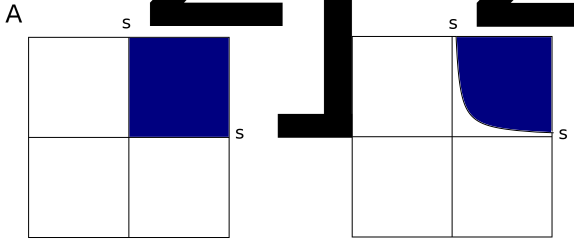
\includegraphics[width=0.7\columnwidth]{fig/region2and3.pdf}
% \caption{{\bf Stability conditions on coefficients of the characteristic polynomial for two and three component systems.} The regions correspond to all possible relationships between the invariants determined by the characteristic polynomial.}
% \label{fig:region2and3}
% \end{figure}

% \pagebreak

% \begin{figure}[!ht]
% \centering
% \noindent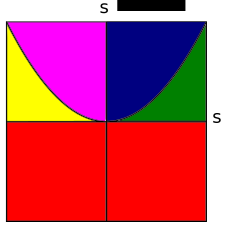
\includegraphics[width=0.5\columnwidth]{fig/region2x2.pdf}
% \caption{{\bf Stability conditions on coefficients of the characteristic polynomial for two component systems.} The regions correspond to all possible relationships between the invariants determined by the characteristic polynomial. Colors correspond to the regions given in the main text Green: $R_{2000}$, Red: $R_{1100}$, Yellow: $R_{0200}$, Magenta: $R_{0002}$, Blue: $R_{0020}$.}
% \label{fig:region2x2}
% \end{figure}

% \pagebreak

% \begin{figure}[!ht]
% \centering
% \noindent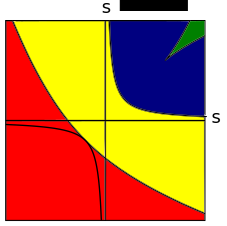
\includegraphics[width=0.5\columnwidth]{fig/region3x3.pdf}
% \caption{{\bf Stability conditions on coefficients of the characteristic polynomial for three component systems.} Colors correspond to the following regions Green: $R_{3000}$, Red: $R_{1200}$, Yellow: $R_{1002}$, Blue: $R_{1020}$. This is the plane $s_3=1$.}
% \label{fig:region3x3}
% \end{figure}

\pagebreak
\FloatBarrier

% \section{Tables}
%!TEX root = ../paper.tex
\newcommand{\specialcell}[2][c]{%
  \begin{tabular}[#1]{@{}c@{}}#2\end{tabular}}

\begin{table}[h]
\begin{center}
\begin{tabular}{ c || c | c | c }
\hline
matrix & connectivity & \specialcell{probability of stability\\to perturbation} & \specialcell{probability\\of stability}\\
\hline
  $\begin{pmatrix}
a & b \\
d & c
\end{pmatrix}$ & 4 & 0.62 & 0.25 \\
  $\begin{pmatrix}
a & b \\
d & 0
\end{pmatrix}$, $\begin{pmatrix}
0 & b \\
d & c
\end{pmatrix}$ & 3 & 0.5 & 0.25 \\
  $\begin{pmatrix}
a & 0 \\
d & c
\end{pmatrix}$, $\begin{pmatrix}
a & b \\
0 & c
\end{pmatrix}$ & 3 & 0.67 & 0.25 \\
$\begin{pmatrix}
a & 0 \\
0 & c
\end{pmatrix}$ & 2 & 0.5 & 0.25 \\
\end{tabular}
\end{center}
\caption{{\bf Probability of stability under resampling and \emph{a priori} stability for two component systems derived analytically}. All matrices not listed have $0$ probability of stability.}\label{tab:structstabmat}
\end{table}

\pagebreak
%!TEX root = ../paper.tex
\begin{longtable}{ c | c || c | c | c | c | c }
\hline
matrix & \specialcell{orbit\\size} & connectivity & \specialcell{edit\\distance} & \specialcell{cycle\\number} & \specialcell{probability of stability\\to perturbation} & \specialcell{probability\\of stability}\\
\hline
$\begin{pmatrix}
1 & 0 & 0\\
0 & 1 & 0\\
0 & 0 & 1\\
\end{pmatrix}$ & 1 & 3 & 3 & 0 & 0.499 & 0.126\\
$\begin{pmatrix}
0 & 0 & 1\\
0 & 1 & 0\\
1 & 0 & 1\\
\end{pmatrix}$ & 6 & 4 & 4 & 1 & 0.505 & 0.121\\
$\begin{pmatrix}
1 & 0 & 0\\
0 & 1 & 1\\
0 & 0 & 1\\
\end{pmatrix}$ & 6 & 4 & 2 & 0 & 0.622 & 0.127\\
$\begin{pmatrix}
0 & 0 & 1\\
0 & 1 & 1\\
1 & 0 & 1\\
\end{pmatrix}$ & 12 & 5 & 3 & 1 & 0.595 & 0.121\\
$\begin{pmatrix}
0 & 0 & 1\\
0 & 1 & 1\\
1 & 1 & 0\\
\end{pmatrix}$ & 6 & 5 & 5 & 2 & 0.494 & 0.128\\
$\begin{pmatrix}
0 & 1 & 1\\
0 & 0 & 1\\
1 & 0 & 1\\
\end{pmatrix}$ & 12 & 5 & 3 & 2 & 0.41 & 0.061\\
$\begin{pmatrix}
0 & 1 & 0\\
0 & 1 & 1\\
1 & 0 & 1\\
\end{pmatrix}$ & 6 & 5 & 3 & 1 & 0.43 & 0.078\\
$\begin{pmatrix}
0 & 1 & 1\\
0 & 1 & 0\\
1 & 0 & 1\\
\end{pmatrix}$ & 12 & 5 & 3 & 1 & 0.605 & 0.12\\
$\begin{pmatrix}
0 & 1 & 1\\
0 & 1 & 1\\
1 & 0 & 0\\
\end{pmatrix}$ & 6 & 5 & 3 & 2 & 0.405 & 0.06\\
$\begin{pmatrix}
1 & 0 & 1\\
0 & 1 & 1\\
0 & 0 & 1\\
\end{pmatrix}$ & 6 & 5 & 1 & 0 & 0.698 & 0.122\\
$\begin{pmatrix}
1 & 0 & 0\\
0 & 1 & 1\\
0 & 1 & 1\\
\end{pmatrix}$ & 3 & 5 & 3 & 1 & 0.587 & 0.128\\
$\begin{pmatrix}
1 & 0 & 1\\
0 & 1 & 0\\
0 & 1 & 1\\
\end{pmatrix}$ & 6 & 5 & 1 & 0 & 0.707 & 0.127\\
$\begin{pmatrix}
0 & 0 & 1\\
0 & 1 & 1\\
1 & 1 & 1\\
\end{pmatrix}$ & 6 & 6 & 4 & 2 & 0.578 & 0.121\\
$\begin{pmatrix}
0 & 1 & 1\\
0 & 0 & 1\\
1 & 1 & 1\\
\end{pmatrix}$ & 6 & 6 & 4 & 3 & 0.487 & 0.081\\
$\begin{pmatrix}
0 & 1 & 1\\
0 & 1 & 1\\
1 & 0 & 1\\
\end{pmatrix}$ & 12 & 6 & 2 & 2 & 0.543 & 0.098\\
$\begin{pmatrix}
0 & 1 & 0\\
0 & 1 & 1\\
1 & 1 & 1\\
\end{pmatrix}$ & 6 & 6 & 2 & 2 & 0.501 & 0.088\\
$\begin{pmatrix}
0 & 1 & 1\\
0 & 1 & 0\\
1 & 1 & 1\\
\end{pmatrix}$ & 12 & 6 & 2 & 1 & 0.662 & 0.123\\
$\begin{pmatrix}
0 & 1 & 1\\
0 & 1 & 1\\
1 & 1 & 0\\
\end{pmatrix}$ & 12 & 6 & 4 & 3 & 0.467 & 0.079\\
$\begin{pmatrix}
0 & 1 & 1\\
1 & 1 & 0\\
1 & 0 & 1\\
\end{pmatrix}$ & 3 & 6 & 4 & 2 & 0.583 & 0.13\\
$\begin{pmatrix}
1 & 0 & 1\\
0 & 1 & 1\\
0 & 1 & 1\\
\end{pmatrix}$ & 12 & 6 & 2 & 1 & 0.659 & 0.124\\
$\begin{pmatrix}
1 & 1 & 1\\
0 & 1 & 1\\
0 & 0 & 1\\
\end{pmatrix}$ & 6 & 6 & 0 & 0 & 0.751 & 0.124\\
$\begin{pmatrix}
1 & 1 & 0\\
0 & 1 & 1\\
1 & 0 & 1\\
\end{pmatrix}$ & 2 & 6 & 2 & 1 & 0.604 & 0.097\\
$\begin{pmatrix}
0 & 1 & 1\\
0 & 1 & 1\\
1 & 1 & 1\\
\end{pmatrix}$ & 12 & 7 & 3 & 3 & 0.564 & 0.103\\
$\begin{pmatrix}
0 & 1 & 1\\
1 & 0 & 1\\
1 & 1 & 1\\
\end{pmatrix}$ & 3 & 7 & 5 & 5 & 0.475 & 0.068\\
$\begin{pmatrix}
0 & 1 & 1\\
1 & 1 & 1\\
1 & 0 & 1\\
\end{pmatrix}$ & 6 & 7 & 3 & 3 & 0.591 & 0.108\\
$\begin{pmatrix}
1 & 1 & 1\\
0 & 1 & 1\\
0 & 1 & 1\\
\end{pmatrix}$ & 6 & 7 & 1 & 1 & 0.717 & 0.119\\
$\begin{pmatrix}
1 & 0 & 1\\
0 & 1 & 1\\
1 & 1 & 1\\
\end{pmatrix}$ & 3 & 7 & 3 & 2 & 0.648 & 0.122\\
$\begin{pmatrix}
1 & 1 & 1\\
0 & 1 & 1\\
1 & 0 & 1\\
\end{pmatrix}$ & 6 & 7 & 1 & 2 & 0.627 & 0.105\\
$\begin{pmatrix}
0 & 1 & 1\\
1 & 1 & 1\\
1 & 1 & 1\\
\end{pmatrix}$ & 3 & 8 & 4 & 5 & 0.577 & 0.093\\
$\begin{pmatrix}
1 & 1 & 1\\
0 & 1 & 1\\
1 & 1 & 1\\
\end{pmatrix}$ & 6 & 8 & 2 & 3 & 0.639 & 0.109\\
$\begin{pmatrix}
1 & 1 & 1\\
1 & 1 & 1\\
1 & 1 & 1\\
\end{pmatrix}$ & 1 & 9 & 3 & 5 & 0.638 & 0.106\\
\caption{{\bf Robustness and stability for three variable systems estimated via Monte Carlo sampling.} All matrices not listed have $0$ probability of stability.}\label{tab:structstabmat3}
\end{longtable}


\end{document}

%------------------------------------------------------------------------------
% End of paper.tex
%------------------------------------------------------------------------------
